\documentclass{MainStyle}

\usepackage{amsthm, amsfonts, amsmath, amssymb, quiver, mathrsfs, newclude, tikz-cd, ctex}

% Customise href Colours.
\usepackage[colorlinks = true,
            linkcolor = blue,
            urlcolor  = blue,
            citecolor = blue,
            anchorcolor = blue]{hyperref}

\newcommand{\changeurlcolor}[1]{\hypersetup{urlcolor=#1}}       

\newcommand*{\name}{张陈成}
\newcommand*{\id}{023071910029}
\newcommand*{\course}{$K$-理论笔记}
\newcommand*{\assignment}{泛函分析拾遗}

\theoremstyle{definition}
\newtheorem{example}{例}

\theoremstyle{definition}
\newtheorem{slogan}{原旨}

\theoremstyle{definition}
\newtheorem{definition}{定义}

\theoremstyle{definition}
\newtheorem{proposition}{命题}

\theoremstyle{definition}
\newtheorem{problem}{问题}

\theoremstyle{definition}
\newtheorem{assumption}{假定}

\theoremstyle{definition}
\newtheorem{theorem}{定理}

\theoremstyle{remark}
\newtheorem{remark}{注}

\theoremstyle{remark}
\newtheorem{lemma}{引理}
\allowdisplaybreaks

\begin{document}
\maketitle
\tableofcontents


\section{Banach 代数的极大理想}

\begin{definition}[Banach 代数]
    称复 Banach 空间 $(X,\|\cdot\|)$ 为 Banach 代数, 若存在 $X$ 上的乘法使得 $\|xy\|\leq \|x\|\cdot \|y\|$.
\end{definition}

\begin{remark}
    不妨假定 Banach 代数有单位元. 实际上, 总可以对具有乘法结构加群添加单位元. 任给 Banach 代数 $(X,\|\cdot\|,\cdot)$, 定义含有单位元的 Banach 代数 $(X\oplus \mathbb C, \| \cdot \|',\odot)$ 如下.
    \begin{itemize}
        \item 范数 $\|(x,z)\|':=\|x\|+|z|$ 满足 $\mathbb C$-线性性与次可加性.
        \item 乘法 $(x,z)\odot(y,w):=(xy+zy+wx,zw)$ 与结合律, 分配律, 范数相容.
        \item 单位元 $(0,1)$ 具有范数 $1$, 且与乘法相容.
    \end{itemize}
    上述单位化过程对交换 Banach 代数亦适用.
\end{remark}

\begin{proposition}[逆元子群]
    Banach 代数的逆元全体 $X^\times$ 为开群, 且 $(-)^{-1}$ 为同胚.
    \begin{proof}
        任取 $x\in X^\times$, 以及 $t\in B(0,\|x^{-1}\|)$, 根据一致收敛性有
        \begin{align*}
            e=(x+t)(x^{-1}-x^{-1}tx^{-1}+x^{-1}tx^{-1}tx^{-1}-\cdots)=(x+t)\cdot x^{-1}\cdot \sum_{n\geq 1}(-tx^{-1})^n.
        \end{align*}
        往证 $(-)^{-1}$ 的连续性. 注意到 $\left|(\|(x+s)^{-1}\|-\|x^{-1}\|)\right|\leq\|x^{-1}\|\cdot |1-\|e+x^{-1}s\||$, 往后仅需验证单位元处逆映射连续. 对足够小的 $s$, 有
        \begin{align*}
            \|e-(e-s)^{-1}\|=\left\|\sum_{n\geq 1} s^n\right\|\leq \dfrac{|s|}{1-\|s\|}.
        \end{align*}
        从而 $(e-s)^{-1}\in B\left(e,\dfrac{|s|}{1-|s|}\right)$. 证毕.
    \end{proof}
\end{proposition}

\begin{definition}[(双边)理想]
    Banach 代数 $X$ 的理想为线性子空间 $I$, 满足 $IX+XI\subseteq I$.
\end{definition}

\begin{proposition}
    真理想之闭包也是真理想. 特别地, 极大理想闭.
    \begin{proof}
        真理想 $I\subsetneqq X$ 中元素不可逆, 从而对任意 $r\in I$ 总有 $\|e-r\|\geq 1$. 显然 $\overline I\subsetneqq X$. 极大理想 $\mathfrak m$ 的存在性由选择公理保证, 再由 $\mathfrak m\subseteq \overline{\mathfrak m}\subsetneqq X$ 知 $\mathfrak m=\overline{\mathfrak m}$.
    \end{proof}
\end{proposition}

\begin{definition}[商代数]
    给定 Banach 代数 $X$ 与理想 $I$, 商代数 $X/I$ 的单位元为 $e+I$, 范数定义作
    \begin{align*}
        \|x+I\|_{X/I}:=\inf_{r\in I}\|x+r\|_X.
    \end{align*}
\end{definition}

\begin{remark}
    商算子 $X\overset \pi \twoheadrightarrow X/I$ 的范数为 $1$.
\end{remark}

\begin{definition}[特征]
    称 $\mathbb C$-代数同态(可乘线性泛函) $\varphi: X\to \mathbb C$ 为特征.
\end{definition}

\begin{proposition}\label{max-ideal}
    特征有如下特性.
    \begin{enumerate}
        \item 特征的范数为 $1$, 且在
              $X^\ast$ 中弱-$\ast$ 紧.
        \item $\varphi$ 是特征, 当且仅当 $\varphi(e)=1$ 与 $\varphi (x^2)=\varphi (x)^2$ 成立.
        \item 特征与极大理想对应.
    \end{enumerate}
    \begin{proof}
        以下依次证明之.
        \begin{enumerate}
            \item 仅需证明对任意 $x\in X$ 均有 $|\varphi (x)|\leq 1$. 若不然, 则存在 $x\in X$ 使得 $e-\dfrac{x}{\varphi(x)}$ 可逆, 但
                  \begin{align*}
                      \varphi \left(e-\dfrac{x}{\varphi(x)}\right)=\varphi (e)-\dfrac{\varphi(x)}{\varphi(x)}=0.
                  \end{align*}
                  这与 $\varphi:X^\times \to \mathbb C^\times $ 矛盾. 对弱-$\ast$ 紧性, Banach-Alaoglu 定理表明 $1$-范数的线性泛函全体弱-$\ast$ 紧, 因此证明全体特征弱-$\ast$ 闭即可. 直接验证之, 显然.
            \item 注意到 $0=\varphi (x+y)^2-\varphi ((x+y)^2)=\varphi (xy+yx)-2\varphi (x)\varphi (y)$, 故 $\varphi$ 与 $\ker(\varphi)$ 相容. 根据
                  \begin{align*}
                      2x(yxy)+2(yxy)x=(xy+yx)^2+(xy-yx)^2,
                  \end{align*}
                  从而 $x\in \ker(\varphi)$ 当且仅当 $(xy\pm yx)\in \ker(\varphi )$, 即 $xy,yx\in \ker(\varphi)$. 遂有
                  \begin{align*}
                      0=\varphi ((x-e\varphi (x))(y-e\varphi (y)))=\varphi(xy)-\varphi (x)\varphi(y),\quad \forall x,y\in X.
                  \end{align*}
            \item 先证明特征 $\varphi _1=\varphi_2$ 当切仅当 $\ker(\varphi_1)=\ker(\varphi_2)$. 往证必要性. 若 $\varphi_1\neq \varphi_2$, 则存在 $x$ 使得 $\varphi_1(x)\neq \varphi_2(x)$. 此时 $x-e\varphi _1(x)$ 为 $\varphi_1$ 的核, 但非 $\varphi_2$ 的核. 遂得证. \par
                  由于 $\dim_{\mathbb C}(X/\varphi_i)=1$, 故 $\ker(\varphi_i)$ 为极大理想. 相反地, 给定任意极大理想 $\mathfrak m\subseteq X$, 则 $X/\mathfrak m$ 为复交换可除 Banach 代数, 因此只能是 $\mathbb C$. 商映射 $X/\mathfrak m$ 自然给出特征. 结合特征到极大理想的典范映射是单的, 因此是一一对应.
        \end{enumerate}
    \end{proof}
\end{proposition}

\section{谱理论}

\begin{definition}[全纯函数]
    对开区域 $\Omega\subseteq \mathbb C$ 与 Banach 代数 $X$, 称 $f:\Omega\to X$ 是全纯的当且仅当极
    \begin{align*}
        \lim_{z\to z_0}\dfrac{f(z)-f(z_0)}{z-z_0}=:f'(z_0)
    \end{align*}
    对任意 $z_0\in \Omega$ 存在.
\end{definition}

\begin{remark}
    若 $X$ 是复拓扑线性空间, 则称 $f:\Omega\to X$ 弱全纯, 当且仅当对任意对偶空间中的线性泛函 $l\in X^\ast$ 总有全纯函数
    \begin{align*}
        l(f):\Omega \to \mathbb C, \quad x\mapsto (l(f))(x)=l(f(x)).
    \end{align*}
    若 $X$ 为复 Banach 空间, 则弱全纯函数等价于全纯函数.
\end{remark}

\begin{proposition}
    类比复分析中证明, 全纯函数 $f:\Omega\to X$ 满足以下性质.
    \begin{enumerate}
        \item $f$ 光滑.
        \item 定义参数化闭道路 $\gamma\subseteq\Omega$ 关于 $z_0\in (\mathbb C\setminus \gamma)$ 的盈数为 $\displaystyle \mathrm{Ind}_\gamma (z_0):=\dfrac{1}{2\pi i}\int_\gamma\dfrac{\mathrm dz}{z-z_0}\in \mathbb Z$.
        \item (Cauchy 定理)若 $\gamma$ 在 $\Omega$ 上零伦, 即, 对任意 $z_0\in (\mathbb C\setminus\Omega)$ 均有 $\mathrm{Ind}_\gamma(z_0)=0$, 则 $\displaystyle \int_\gamma f(z)\mathrm dz=0$.
        \item (Cauchy 积分公式)对任意参数化闭曲线 $\gamma$ 与 $z_0\in (\Omega\setminus \gamma)$, 总有
              \begin{align*}
                  \mathrm{Ind}_\gamma(z_0)\cdot f(z_0) =\int_\gamma \dfrac{f(z)}{z-z_0}\,\mathrm dz.
              \end{align*}
        \item (Liouville 定理)取 $Y\subseteq X^\ast$ 分离 $X$, 若对任意 $l\in Y$, $l(f):\mathbb C\to \mathbb C$ 有界, 则 $f$ 是常映射.
    \end{enumerate}
\end{proposition}

\begin{definition}[谱]
    给定 Banach 代数 $X$, 定义 $x\in X$ 的谱为
    \begin{align*}
        \sigma(x):=\{z\in \mathbb C\mid (z e-x)\notin X^\times \}.
    \end{align*}
\end{definition}

\begin{theorem}
    $\sigma(x)\in \overline{B(0,\|x\|)}$, 且 $\sigma$ 为非空闭集.
    \begin{proof}
        对任意 $|z|>\|x\|$ 有 $ze-x=ze(1-z^{-1}x)$. 注意到 $\|z^{-1}x\|<1$, 故 $x$ 可逆, 从而 $\sigma(x)\subseteq \overline{B(0,\|x\|)}$. 作连续函数 $T_x:=(\cdot)e-x:\mathbb C\to X$, 从而闭集 $(X\setminus X^\times)\cap T_x(\mathbb C)$ 的原像仍是闭集. 最后证明 $\sigma(x)$ 非空, 若不然, 则 $\|(ze-x)^{-1}\|$ 在 $\mathbb C$ 上定义. 注意到 $\lim_{z\to \infty}|z|^{-1}\|(e-z^{-1}x)^{-1}\|=0$, 从而 $(ze-x)^{-1}$ 一致有界. 依照 Liouville 定理, $ze-x$ 为常数算子, 矛盾.
    \end{proof}
\end{theorem}

\begin{definition}[广义幂零元]
    根据 Laurent 展开直接验证得幂零元的谱为 $\{0\}$;相应地, 称谱为 $\{0\}$ 的元素为\textbf{广义幂零元}.
\end{definition}

\begin{definition}[谱半径]
    定义 $x\in X$ 的\textbf{谱半径}为紧集 $\sigma(x)$ 中模长最大者, 记 $r(x)$.
\end{definition}

\begin{proposition}
    $r(x)=\lim_{n\to\infty}\sqrt[n]{\|x^n\|}$.
    \begin{proof}
        一方面, $r(x)\leq \liminf_{n\to\infty}\sqrt[n]{\|x^n\|}$ 是显然的. 另一方面, 有 Laurent 展开
        \begin{align*}
            (ez-x)^{-1}=\sum_{n\geq 0} z^{-{n+1}}x^n\quad (|z|>r(x)).
        \end{align*}
        以上收敛半径为 $\limsup_{n\to\infty}\|z^{-1-n}x^n\|\leq 1$, 从而 $r(x)\geq \lim\sup_{n\to\infty}\sqrt[n+1]{\|x^n\|}$. 综上, 得证.
    \end{proof}
\end{proposition}

\begin{remark}
    $r:X\to \mathbb R_{\geq 0}$ 上半连续, 即, 对一切依范数收敛的序列 $x_n\to x$ 总有
    \begin{align*}
        \limsup_{n\to\infty} r(x_n)\leq r(x).
    \end{align*}
\end{remark}

\begin{remark}
    谱可以定义在一般 $X$-算子上, 其中 $x:X\to X, y\mapsto xy$ 自然是 Banach 空间的算子. 归根结底, 算子代数也是 Banach 代数.
\end{remark}

\begin{proposition}\label{Banach-extension}
    对 Banach 代数 $X$ 与子代数 $Y$, 定义
    \begin{align*}
        G(X):=\{(x,z)\in X\times \mathbb C\mid z\notin \sigma_X(x)\}.
    \end{align*}
    则 $G(Y)$ 无非 $G(X)\cap (\mathbb C\times Y)$ 去掉若干连通分支, 且数量不超过 $\omega \cdot \dim _{\mathbb C}Y$.
    \begin{center}
        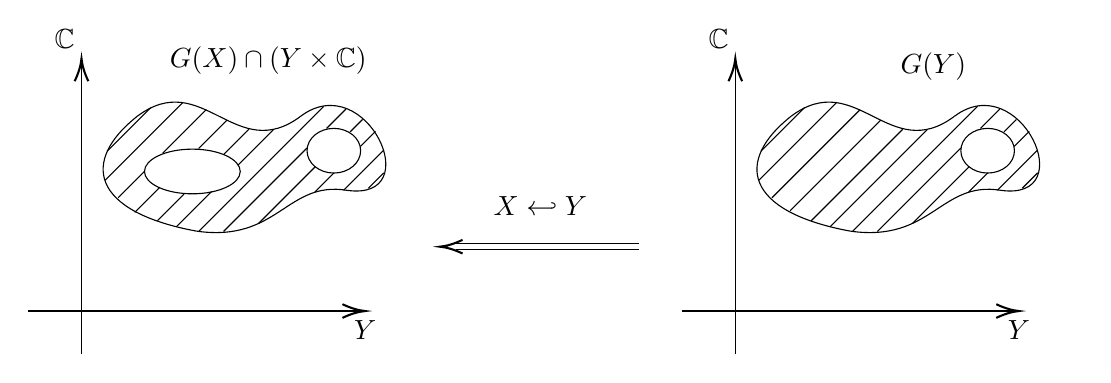
\begin{tikzpicture}[x=0.75pt,y=0.75pt,yscale=-1,xscale=1]
            %uncomment if require: \path (0,177); %set diagram left start at 0, and has height of 177

            %Straight Lines [id:da9161134884051503] 
            \draw    (85,150) -- (245.33,150) ;
            \draw [shift={(247.33,150)}, rotate = 180] [color={rgb, 255:red, 0; green, 0; blue, 0 }  ][line width=0.75]    (10.93,-3.29) .. controls (6.95,-1.4) and (3.31,-0.3) .. (0,0) .. controls (3.31,0.3) and (6.95,1.4) .. (10.93,3.29)   ;
            %Straight Lines [id:da982834457118575] 
            \draw    (110.67,170.83) -- (110.67,30.33) ;
            \draw [shift={(110.67,28.33)}, rotate = 90] [color={rgb, 255:red, 0; green, 0; blue, 0 }  ][line width=0.75]    (10.93,-3.29) .. controls (6.95,-1.4) and (3.31,-0.3) .. (0,0) .. controls (3.31,0.3) and (6.95,1.4) .. (10.93,3.29)   ;
            %Curve Lines [id:da11499090372454934] 
            \draw    (137.55,56.15) .. controls (169.04,32.53) and (184.78,79.77) .. (216.27,56.15) ;
            %Curve Lines [id:da6543975363696191] 
            \draw    (216.27,56.15) .. controls (247.76,32.53) and (277.93,97.35) .. (238.57,91.84) ;
            %Curve Lines [id:da2672262975077062] 
            \draw    (238.57,91.84) .. controls (209.45,87.11) and (205.51,117.03) .. (166.15,111.52) ;
            %Curve Lines [id:da3984131535722564] 
            \draw    (137.55,56.15) .. controls (110.26,77.67) and (114.98,102.07) .. (166.15,111.52) ;

            %Shape: Ellipse [id:dp20836044364640283] 
            \draw   (141,82.76) .. controls (141,76.82) and (151.33,72) .. (164.08,72) .. controls (176.82,72) and (187.15,76.82) .. (187.15,82.76) .. controls (187.15,88.7) and (176.82,93.52) .. (164.08,93.52) .. controls (151.33,93.52) and (141,88.7) .. (141,82.76) -- cycle ;
            %Shape: Ellipse [id:dp9235609515993308] 
            \draw   (219.33,72.76) .. controls (219.33,66.82) and (225.11,62) .. (232.24,62) .. controls (239.37,62) and (245.15,66.82) .. (245.15,72.76) .. controls (245.15,78.7) and (239.37,83.52) .. (232.24,83.52) .. controls (225.11,83.52) and (219.33,78.7) .. (219.33,72.76) -- cycle ;
            %Straight Lines [id:da46138281028473904] 
            \draw    (122,87) -- (159.33,49.67) ;
            %Straight Lines [id:da5497744393131812] 
            \draw    (123,73) -- (144,52) ;
            %Straight Lines [id:da9741406223503668] 
            \draw    (149.76,74) -- (170.76,53) ;
            %Straight Lines [id:da40280557780431736] 
            \draw    (128.33,95.43) -- (141,82.76) ;
            %Straight Lines [id:da14075024833671357] 
            \draw    (167.09,71.67) -- (180.76,58) ;
            %Straight Lines [id:da17717679565144473] 
            \draw    (136.33,102.43) -- (148.33,90.43) ;
            %Straight Lines [id:da9476206918339021] 
            \draw    (179.33,74.43) -- (191.33,62.43) ;
            %Straight Lines [id:da12666277080293287] 
            \draw    (147.33,106.43) -- (160.08,93.68) ;
            %Straight Lines [id:da960198955345378] 
            \draw    (186.09,79.67) -- (203.08,62.68) ;
            %Straight Lines [id:da4946816819630324] 
            \draw    (156.33,109.43) -- (173.33,92.43) ;
            %Straight Lines [id:da1709001090943063] 
            \draw    (167.09,111.67) -- (227.33,51.43) ;
            %Straight Lines [id:da4298213050058375] 
            \draw    (179.09,111.67) -- (219.33,71.43) ;
            %Straight Lines [id:da7274559958614968] 
            \draw    (228.76,62) -- (238.09,52.67) ;
            %Straight Lines [id:da3330655605485695] 
            \draw    (196.09,107.67) -- (223.33,80.43) ;
            %Straight Lines [id:da4106084639939238] 
            \draw    (240.09,63.67) -- (246.09,57.67) ;
            %Straight Lines [id:da8648280177673044] 
            \draw    (223.09,92.67) -- (232.24,83.52) ;
            %Straight Lines [id:da7603389763374122] 
            \draw    (245,70.76) -- (252.33,63.43) ;
            %Straight Lines [id:da5853101991327216] 
            \draw    (236.92,91.84) -- (256.33,72.43) ;
            %Straight Lines [id:da5521095956648154] 
            \draw    (248.92,90.84) -- (256.33,83.43) ;
            %Straight Lines [id:da5574132708658619] 
            \draw    (400,150) -- (560.33,150) ;
            \draw [shift={(562.33,150)}, rotate = 180] [color={rgb, 255:red, 0; green, 0; blue, 0 }  ][line width=0.75]    (10.93,-3.29) .. controls (6.95,-1.4) and (3.31,-0.3) .. (0,0) .. controls (3.31,0.3) and (6.95,1.4) .. (10.93,3.29)   ;
            %Straight Lines [id:da8261829163991603] 
            \draw    (425.67,170.83) -- (425.67,30.33) ;
            \draw [shift={(425.67,28.33)}, rotate = 90] [color={rgb, 255:red, 0; green, 0; blue, 0 }  ][line width=0.75]    (10.93,-3.29) .. controls (6.95,-1.4) and (3.31,-0.3) .. (0,0) .. controls (3.31,0.3) and (6.95,1.4) .. (10.93,3.29)   ;
            %Curve Lines [id:da3319259495653488] 
            \draw    (452.55,56.15) .. controls (484.04,32.53) and (499.78,79.77) .. (531.27,56.15) ;
            %Curve Lines [id:da814431271966354] 
            \draw    (531.27,56.15) .. controls (562.76,32.53) and (592.93,97.35) .. (553.57,91.84) ;
            %Curve Lines [id:da2888860467131018] 
            \draw    (553.57,91.84) .. controls (524.45,87.11) and (520.51,117.03) .. (481.15,111.52) ;
            %Curve Lines [id:da26828656957672803] 
            \draw    (452.55,56.15) .. controls (425.26,77.67) and (429.98,102.07) .. (481.15,111.52) ;

            %Shape: Ellipse [id:dp3097421098469644] 
            \draw   (534.33,72.76) .. controls (534.33,66.82) and (540.11,62) .. (547.24,62) .. controls (554.37,62) and (560.15,66.82) .. (560.15,72.76) .. controls (560.15,78.7) and (554.37,83.52) .. (547.24,83.52) .. controls (540.11,83.52) and (534.33,78.7) .. (534.33,72.76) -- cycle ;
            %Straight Lines [id:da8415449486335036] 
            \draw    (437,87) -- (474.33,49.67) ;
            %Straight Lines [id:da354096026397162] 
            \draw    (438,73) -- (459,52) ;
            %Straight Lines [id:da8699887187661282] 
            \draw    (443.33,95.43) -- (485.76,53) ;
            %Straight Lines [id:da5155307727372422] 
            \draw    (452.09,101.67) -- (495.76,58) ;
            %Straight Lines [id:da9263975659042796] 
            \draw    (462.09,106.67) -- (506.33,62.43) ;
            %Straight Lines [id:da48746680708821644] 
            \draw    (471.33,109.43) -- (518.08,62.68) ;
            %Straight Lines [id:da7373435763115916] 
            \draw    (482.09,111.67) -- (542.33,51.43) ;
            %Straight Lines [id:da6485844719374732] 
            \draw    (494.09,111.67) -- (534.33,71.43) ;
            %Straight Lines [id:da3309128649954429] 
            \draw    (543.76,62) -- (553.09,52.67) ;
            %Straight Lines [id:da8871564947255322] 
            \draw    (511.09,107.67) -- (538.33,80.43) ;
            %Straight Lines [id:da49133047947096564] 
            \draw    (555.09,63.67) -- (561.09,57.67) ;
            %Straight Lines [id:da4381861607396125] 
            \draw    (538.09,92.67) -- (547.24,83.52) ;
            %Straight Lines [id:da8548434782935674] 
            \draw    (560,70.76) -- (567.33,63.43) ;
            %Straight Lines [id:da47438750580990496] 
            \draw    (551.92,91.84) -- (571.33,72.43) ;
            %Straight Lines [id:da34161459879064293] 
            \draw    (563.92,90.84) -- (571.33,83.43) ;
            %Straight Lines [id:da5530653794769163] 
            \draw    (291.33,117.5) -- (379.33,117.5)(291.33,120.5) -- (379.33,120.5) ;
            \draw [shift={(283.33,119)}, rotate = 0] [color={rgb, 255:red, 0; green, 0; blue, 0 }  ][line width=0.75]    (10.93,-3.29) .. controls (6.95,-1.4) and (3.31,-0.3) .. (0,0) .. controls (3.31,0.3) and (6.95,1.4) .. (10.93,3.29)   ;

            % Text Node
            \draw (247.33,153.4) node [anchor=north] [inner sep=0.75pt]    {$Y$};
            % Text Node
            \draw (108.67,24.93) node [anchor=south east] [inner sep=0.75pt]    {$\mathbb{C}$};
            % Text Node
            \draw (562.33,153.4) node [anchor=north] [inner sep=0.75pt]    {$Y$};
            % Text Node
            \draw (423.67,24.93) node [anchor=south east] [inner sep=0.75pt]    {$\mathbb{C}$};
            % Text Node
            \draw (152,21.4) node [anchor=north west][inner sep=0.75pt]    {$G( X) \cap ( Y\times \mathbb{C})$};
            % Text Node
            \draw (504,24.4) node [anchor=north west][inner sep=0.75pt]    {$G( Y)$};
            % Text Node
            \draw (308,93.4) node [anchor=north west][inner sep=0.75pt]    {$X\hookleftarrow Y$};
        \end{tikzpicture}
    \end{center}
    \begin{proof}
        将证明拆解为如下步骤.
        \begin{enumerate}
            \item 对任意 $y\in Y$, 有 $\partial \sigma_Y(y)\subseteq \sigma_X(y)\subseteq \sigma_Y(y)$. 于是 $\sigma_Y(y)$ 无非 $\sigma_X(y)$ 填上若干开连通分支.
            \item 任意给定 $\sigma_X(x)$, 则对任意小的 $\varepsilon$-网 $\bigcup_{t\in \sigma_X(x)}B(t,\varepsilon)$, 存在 $\delta$ 使得对任意 $\|y\|< 1$ 均有
                  \begin{align*}
                      \sigma_X(x+\delta y)\subseteq \bigcup_{t\in \sigma_X(x)}B(t,\varepsilon).
                  \end{align*}
                  换言之, $\sigma_X(-)$ 关于 $\varepsilon$-网诱导的度量连续. 记上述 $\varepsilon$-网作 $N_\varepsilon$.
        \end{enumerate}
        对第一部分, $\sigma_X(y)\subseteq \sigma_Y(y)$ 是显然的, 因为 $Y^\times \subseteq X^\times$. 对任意 $z_0\in \partial\sigma_Y(y)$, 存在道路
        \begin{align*}
            z:[0,1]\to \mathbb C, \quad (0,1]\to \mathbb C\setminus \sigma_Y(y),\quad 0\mapsto z_0.
        \end{align*}
        因此对 $t\in (0,1]$, $(z(t)e-y)^{-1}\in Y^\times \subseteq X^\times$. 若 $z_0\notin \sigma_X(y)$, 则根据 $(-)^{-1}$ 的连续性知 $(z_0e-y)^{-1}\in X^\times$. 注意到 $Y$ 是 $X$ 的闭子空间, 故 $\{(z(t)e-y)^{-1}\mid t\in [0,1]\}$ 的原像均在 $Y$ 中. 显然 $(z_0e-y)^{-1}\in Y$ 有逆元 $(z_0r-y)\in Y$. \par
        对第二部分, 考虑连续映射 $N:\mathbb C\setminus \sigma_X(x)\to \mathbb R, \quad z\mapsto \|(ze-x)^{-1}\|$. 显然 $N(\infty)=0$, 故 $N$ 在 $\mathbb C\setminus N_\varepsilon$ 中有上界 $M$. 根据 $(-)^{-1}$ 与 $\|\cdot\|$ 之连续性, 存在 $\delta =M^{-1}$ 使得对任意 $\|x'-x\|<\delta$ 与 $z\in \mathbb C\setminus N_\varepsilon$, 总有
        \begin{align*}
            \|(ze-x)-(ze-x')\|<\delta \leq \dfrac{1}{\|(ze-x)^{-1}\|}.
        \end{align*}
        因此 $1>\|e-(ze-x)^{-1}(ze-x')\|$. 这也说明
        \begin{align*}
            e-\Big(e-(ze-x)^{-1}(ze-x')\Big)=(ze-x)^{-1}(ze-x')\in X^\times.
        \end{align*}
        对一切 $y\in Y$, 步骤一中填充的连通分支数量至多可数, 从而 $G(Y)$ 与 $G(X)\cap (\mathbb C\times Y)$ 相差的连通分支数不超过 $\omega \cdot \dim_{\mathbb C}Y$.
    \end{proof}
\end{proposition}

\section{$C^\ast$ 代数一览}

\begin{definition}[伴随, Banach$^\ast$ 代数]
    Banach 代数 $X$ 上的\textbf{伴随}为 $\mathbb R$-反自同构 $(-)^\ast:X\to X$, 满足
    \begin{align*}
        (z\cdot x)^\ast=\overline z x^\ast,\quad (x^\ast)^\ast=x.
    \end{align*}
    称具有伴随的 Banach 代数为 \textbf{Banach$^\ast$ 代数}.
\end{definition}

\begin{proposition}
    自伴元全体 $\{x=x^\ast\mid x\in X\}$ 为包含 $e$ 的 $X$ 的实子空间.
\end{proposition}

\begin{proposition}
    $x$ 可逆当且仅当 $x^\ast$ 可逆, 且 $(x^{-1})^\ast=(x^\ast)^{-1}$, $\sigma_X(x)$ 与 $\sigma_X(x^\ast)$ 共轭.
    \begin{proof}
        注意到 $(ze-x)^\ast ((ze-x)^{-1})^\ast=((ze-x)^{-1}(ze-x))^\ast=e^\ast=e$. 从而 $\sigma_X(x)$ 与 $\sigma_X(x^\ast)$ 共轭. 考虑 $z=0$, 则 $x\in X^\times$ 当且仅当 $x^\ast \in X^\times$.
    \end{proof}
\end{proposition}

\begin{definition}[$C^\ast$ 代数]
    称 Banach$^\ast$ 代数为 $C^\ast$ 代数, 当且仅当 $(-)^\ast$ 等距.
\end{definition}

\begin{remark}
    对一般交换 Banach 代数, $(-)^\ast$ 等距当且仅当 $\|xx^\ast\|=\|x^\ast x\|=\|x\|^2=\|x^2\|$.
\end{remark}

\begin{proposition}[$C^\ast$ 代数的单位化]
    对非单位 $C^\ast$ 代数 $X$ $\textcolor{red}{\text{未完待续}}$.
\end{proposition}

\begin{definition}[正规元, 酉元, 自伴元(实元)]
    称 $x\in X$ 正规, 若且仅若 $x^\ast x=xx^\ast$; 称 $x$ 是酉的, 若且仅若 $x^\ast x=xx^\ast =e$; 称 $x$ 是自伴的(实的)若且仅若 $x=x^\ast$.
\end{definition}

\begin{proposition}[$C^\ast$ 代数中正规元, 酉元, 实元的谱]
    正规元满足 $r(x)=\|x\|$. 酉元的谱为 $S^1$ 中的若干闭弧(点), 实元的谱为 $\mathbb R$ 中的有限闭集之并.
    \begin{proof}
        显然 $r(x)\leq \|x\|$. 注意到
        \begin{align*}
            \|x^{2^n}\|=\sqrt{\|(x^\ast)^{2^n}x^{2^n}\|}=\sqrt{\|(x^\ast x)^{2^n}\|}\leq \sqrt{\|x^\ast x\|}^{2^n}=\|x\|^{2^n},
        \end{align*}
        从而 $r(x)\geq \limsup_{n\to \infty}\|x^{2^n}\|^{2^{-n}}=\|x\|$. 因此 $r(x)=\|x\|$. 从而酉元的谱在单位闭圆盘内, 且关于共轭运算封闭, 因此在 $S^1$ 上. 结合紧性知酉元的谱为 $S^1$ 上有限闭圆弧(点)之并. 给定实元 $x$, 收敛幂级数定义的 $\exp(ix)$ 是酉元. 对任意 $z\in \sigma_X(x)$, 往证 $\exp(iz)$ 为 $\exp(ix)$ 的谱. 注意到
        \begin{align*}
            \exp(iz)-\exp(ix)=(ze-x)\left(\sum_{n\geq 1}\dfrac{i^n}{n!}\sum_{0\leq k\leq n} z^kx^{n-k}\right)=:(ze-x)T.
        \end{align*}
        显然 $T$ 可逆, 从而 $\sigma_X(\exp(iz))=\exp(i\sigma_X(z))\in S^1$. 这表明实元的谱在 $\mathbb R$ 中, 结合紧性知谱为有限闭区间之并.
    \end{proof}
\end{proposition}

\begin{remark}
    一般地, 全纯函数保持谱. 即, 对一切定义在 $\sigma_X(x)$ 的某个 $\varepsilon$ 网上的全纯函数 $f$ 总有 $f(\sigma_X(x))=\sigma_X(f(x))$.
\end{remark}

\begin{proposition}\label{kerx=kerx*x}
    取 Banach$^\ast$ 代数中任意元 $x$, 总有 $\mathrm{ker}(x)=\mathrm{ker}(x^\ast x)$.
    \begin{proof}
        $xy=0\implies y^\ast x^\ast xy=0\implies (xy)^\ast(xy) =0\implies xy=0$.
    \end{proof}
\end{proposition}

\begin{proposition}
    在命题 \ref{Banach-extension} 中置 $X$ 与 $Y$ 为 $C^\ast$ 代数, 则 $G(Y)=G(X)\cap (\mathbb C\times Y)$.
    \begin{proof}
        对任意 $x\in Y$, 往证 $x\in Y^\times$ 当且仅当 $x\in X^\times$. 对任意 $x\in Y$, 实元的谱 $\sigma_Y(x^\ast x)$ 内部为空, 根据命题 \ref{Banach-extension} 知 $\sigma_X(x^\ast x)=\sigma_Y(x^\ast x)$. 结合命题 \ref{kerx=kerx*x} 知 $x^\ast \in X^\times $ 当且仅当 $x^\ast \in Y^\times$. 得证.
    \end{proof}
\end{proposition}

\begin{remark}
    $C^\ast$ 代数扩张不改变谱.
\end{remark}

\section{Gel'fand 对偶}

\begin{definition}[Gel'fand 变换]\label{Gel'fand}
    定义极大理想空间 $\mathfrak M$ 为赋予弱-$\ast$ 拓扑的特征全体, 则 $\mathfrak M$ 是紧的. 依照命题 \ref{max-ideal} 等同极大理想与特征. 定义 Gel'fand 变换为如下线性映射
    \begin{align*}
        \widehat{(-)}:X\to C(\mathfrak M),\quad x\mapsto [\mathfrak M\to \mathbb C,\quad \varphi \mapsto \varphi (x)].
    \end{align*}
\end{definition}

\begin{proposition}
    若 $X$ 是交换 Banach 代数, 则有如下命题.
    \begin{enumerate}
        \item $\overline{(-)}$ 是交换 Banach 代数的连续同态, 且范数为 $1$.
        \item $\ker \widehat{(-)}=J(X)=\bigcap _{\mathfrak m\in \mathfrak M}\mathfrak m$ 为 Jacobson 根.
        \item $\widehat x:\mathfrak M\to \sigma_X(x),\quad \varphi\to \varphi (x)$ 给出交换 Banach 代数与谱的对应.
        \item $\|\widehat x\|:=\sup_{\varphi \in \mathfrak M}|\varphi (x)|=r(x)$.
        \item 以下关于复半单交换 Banach 代数 $X$ 的论断等价.
              \begin{enumerate}
                  \item $J(X)=0$. 根据以上, $\widehat{(-)}$ 是交换 Banach 代数范畴的单态射.
                  \item $\mathfrak M$ 分离 $X$. 即, 对任意不相等的 $x,y\in X$, 总存在 $\varphi \in \mathfrak M$ 使得 $\varphi(x)\neq \varphi(y)$.
                  \item 谱半径 $r(-)$ 为范数. 换言之, $X$ 中不存在非零的广义幂零元.
              \end{enumerate}
        \item $\widehat{(-)}:X\to C(\mathfrak M)$ 等距当且仅当 $\|x^2\|=\|x\|^2$.
    \end{enumerate}
    \begin{proof}
        下依次证明之.
        \begin{enumerate}
            \item 注意到 $\widehat{xy}(\varphi)=\varphi (xy)=\varphi(x)\varphi(y)=\widehat{x}(\varphi)\widehat{y}(\varphi)$, $\widehat{e}=1$, 故 $\widehat{(-)}$ 为同态. 由于特征范数为 $1$, 故 $\widehat X$ 的范数满足
                  \begin{align*}
                      \|\widehat{x}\|:=\sup_{\varphi\in \mathfrak M}|\varphi(x)|\leq \|x\|.
                  \end{align*}
                  从而 $\|\widehat{(-)}\|\leq 1$. 考虑单位元知 $\|\widehat{(-)}\|=1$.
            \item 注意到 $\widehat r=0$ 当且仅当 $\varphi (r)=0$ 对任意 $\varphi\in \mathfrak M$ 成立, 故当且仅当 $r\in J(X)$.
            \item 一方面, 对任意 $\varphi\in \mathfrak M$, 总有 $\varphi:(\varphi (x)e-x)\mapsto 0$, 从而 $\varphi(x)\in \sigma_X(x)$. 另一方面, 对任意 $z\in \sigma(x)$, 考虑包含不可逆元 $ze-x$ 的极大理想即可.
            \item 根据上一条, $\|\hat x\|=\sup_{\varphi \in \mathfrak M}|\varphi (x)|=\sup_{z\in \sigma(x)}=|z|=r(x)$.
            \item 对任意 $(x-y)\in J(X)$, 总有 $\varphi (x)=\varphi(y)$ 对一切 $\varphi\in \mathfrak M$ 成立, 因此 (a) 与 (b) 等价. 若非 (b), 则存在非零的 $x$ 使得 $\|\widehat x\|=r(x)=0$, 遂得非 (c). 既证 $\|\hat x\|=r(x)$ 是良定义的范数, 从而 (b) 蕴含 (c).
            \item 一方面, 若 $\|\widehat x\|=\|x\|$ 恒成立, 则依照 $\widehat{x\cdot x}(\varphi)=(\widehat x(\varphi))^2$ 可知 $\|x^2\|=\|\widehat x^2\|=\|\widehat x\|^2=\|x\|^2$. 另一方面, 若 $\|x^2\|=\|x\|^2$, 则有
                  \begin{align*}
                      \|\widehat x\|=r(x)=\lim_{n\to \infty}\sqrt[n]{x^n}=\lim_{n\to \infty}\sqrt[2^n]{\|x^{2^n}\|}=\lim_{n\to \infty}\sqrt[2^n]{\|x\|^{2^n}}=\|x\|.
                  \end{align*}
        \end{enumerate}
    \end{proof}
\end{proposition}

\begin{remark}
    上述第 5 条 (b) 表明全体特征(极大理想)有自然的紧 Hausdorff 拓扑.
\end{remark}

\begin{proposition}
    记 $C(K)$ 为紧 Hausdorff 空间上的连续复函数全体, 则 $\|\cdot \|:=\|\cdot \|_{\infty}$ 给出复 Banach 代数结构. 则极大理想空间 $\mathfrak M$ 与 $K$ 无异. 实际上, $C(X)$ 中极大理想形如 $\ker(g\mapsto g(x_0))$. 遂有同构
    \begin{align*}
        \widehat{(-)}: C(K)\overset\sim\longrightarrow C(\mathfrak M),\quad f\mapsto [\ker (g\mapsto g(x_0))\mapsto f(x_0)].
    \end{align*}
    \begin{proof}
        先证明 $C(X)$ 中的极大理想形如 $\ker(g\mapsto g(x_0))$. 记 $\mathfrak m_{x_0}=\ker(g\mapsto g(x_0))$, 则 $C(X)/\mathfrak m_{x_0}=\mathbb C$ 是域, 从而 $\mathfrak m_{x_0}$ 是极大理想. 若存在极大理想 $\mathfrak m$ 与形如 $\mathfrak m_{x_0}$ 的理想不同, 则对任意 $x\in X$, 总存在 $l_x\in \mathfrak m$ 使得 $l_x(x)=1$. 遂得开覆盖 $\{\mathrm{supp}(l_x)\}_{x\in X}$, 记 $\{\mathrm{supp}(l_{x_k})\}_{1\leq k \leq n}$ 为有限子覆盖. 注意到
        \begin{align*}
            \left(\sum_{1\leq k\leq n} |f_{x_k}(x)|^2 \right)\in (C(X))^\times \cap \mathfrak m,
        \end{align*}
        从而 $\mathfrak m$ 中理想包含可逆元, 与假定矛盾.
    \end{proof}
\end{proposition}

\begin{theorem}[Gel'fand 对偶]
    交换 $C^\ast$ 代数范畴与紧 Hausdorff 空间范畴范畴等价.
    \begin{proof}
        先证明定义 \ref{Gel'fand} 给出交换 $C^\ast$ 代数 $X$ 到极大理想空间 $C(\mathfrak M)$ 的等距同构, 且保持 $(-)^\ast$. 注意到
        \begin{align*}
            \widehat{x^\ast}: \varphi\mapsto \varphi (x^\ast)=\overline{\varphi (x)},\quad \overline{\widehat x}:[\varphi \mapsto \overline{\varphi(x)}].
        \end{align*}
        从而 $\widehat{(-)}$ 为保持 $(-)^\ast$ 的同态.
    \end{proof}
\end{theorem}

$\textcolor{red}{\text{未完待续}}$.
% https://ncatlab.org/nlab/show/Gelfand+duality

\begin{theorem}[Riez 算法]
    $\textcolor{red}{\text{未完待续}}$.
\end{theorem}

\end{document}